\documentclass{eceasst}

\usepackage{minted}
\usepackage{subfig}
\input{frontmatter}

\usepackage{pdfcomment}
\newcommand{\todo}[1]{\pdfcomment[color={0.045 0.278 0.643},icon=Note]{#1}}

\title{Improving reproducibility of scientific software using Nix/NixOS: A case study on preCICE adapters and solvers}
\short{TODO}
\author{
Max Hausch\autref{1+},
Simon Hauser\autref{2+},
Benjamin Uekermann\autref{3}}

\institute{
\autlabel{1} \email{st175425@stud.uni-stuttgart.de}\\
\autlabel{2} \email{st148883@stud.uni-stuttgart.de}\\
\autlabel{3} \email{Benjamin.Uekermann@ipvs.uni-stuttgart.de}\\
\autlabel{+} These authors contributed equally to this work.}

\abstract{
Ensuring the reproducibility of scientific software is crucial for the advancement of research and the validation of scientific findings.
However, achieving reproducibility in software-intensive scientific projects is often challenging due to dependencies, system configurations and software environments.
In this paper, we present a possible solution for these challenges by utilizing Nix and NixOS.
Nix is a package manager and functional language that allows to mitigate these problems by guaranteeing that a package and all its dependencies can be built reproducibly as long as there is a build plan at the desired time.
NixOS is a purely functional Linux distribution, built on top of Nix that enables the build of reproducible systems including configuration files, packages and their dependencies.
We present a case study on improving the reproducibility of preCICE, an open-source coupling library, and some of its main adapters using Nix and NixOS.
Using this approach, we demonstrate how to create a reproducible and self-contained environment for preCICE and highlight the benefits of using Nix and NixOS for managing software and system configurations, resulting in improved reproducibility.
In addition, we compare the usability and reproducibility provided by Nix, in the context of preCICE, with two already established high-performance computing (HPC) solutions, Spack and EasyBuild.
This evaluation enables us to assess the advantages and disadvantages of employing Nix to improve reproducibility in scientific software development within an HPC context.}

\keywords{Reproducibility, Nix, NixOS, Spack, EasyBuild, preCICE, HPC}

\begin{document}
\maketitle

\section{Introduction}

In scientific research, it's crucial to be able to reproduce and verify results.
Reproducibility ensures that experiments can be repeated and findings can be validated, which is essential for reliable and credible research.
Being able to replicate experiments and computations is important for verifying scientific claims.
However, achieving reproducibility in scientific software has been a challenge due to complex dependencies, conflicting software environments, and changing software systems.
Problems arise from dependencies, library versions, and system configurations, leading to inconsistencies across different computing environments.
Traditional approaches to reproducibility, such as manual setup instructions or virtualization techniques, are prone to errors and time-consuming at best.
It is not scalable and highly inefficient to make every researcher to tediously recreate the exact same environment with traditional approaches.
This calls for a more efficient and automated solution.

Attempts were made to solve this situation by using Docker\footnote{\url{https://www.docker.com/}}, a software which describes software environments with the help of text files.
Those text files are made up of imperative commands which are run inside of containers, one layer at a time.
The result are several different layers which are all combines into a single output image that can be instantiated to a running container.
Docker images can be copied to different hosts and should then provide the same environment on different machines.
An issue that arises here, is that usually those images are based on one of the official Docker images\footnote{\url{https://docs.docker.com/trusted-content/official-images/}} all of which bring traditional package managers like \texttt{apt}.
When a user specifies to install the \texttt{python3} package with a traditional package manager today, the package manager could yield python3.8, whereas running the same command two months from now could yield python in the version 3.9.
This could potentially lead to different results when a user wants to only add a single dependency but has to rebuild the whole image, thus rendering it useless in terms of reproducibility.

In the past years, the Nix package manager~\cite{Dolstra_2004} and NixOS~\cite{Dolstra_2010}, a Linux distribution built around it, have emerged as promising solutions to address these challenges.
This paper explores the use of Nix/NixOS to improve the reproducibility of scientific software.

Conducting a large scale research on building scientific codes reproducibly is quite infeasible due to how many different software there is.
Therefore, we conduct a case study, focusing on preCICE~\cite{preCICEv2}, its adapters and solvers.
One of the goals of the case study is to get a first hand experience and estimate on the complexity and possible challenges when packaging scientific software.
Also, consistent portability of building the software on three different systems is verified.
preCICE is a well fit for such a case study, as its official adapters and solvers vary in their programming languages, project sizes and other factors, providing a quite manifold set of scientific simulation software while still being able to verify if the software is still correct by running preCICE simulations across several different solver binaries.

In high-performance computing (HPC), where performance and efficiency are critical, managing software dependencies and configurations becomes even more challenging.
By using Nix, researchers and practitioners in HPC could easily reproduce computational experiments, ensuring that the same software stack, libraries, and configurations are utilized consistently.
Reproducibility of scientific results can be achieved using the Nix package manager as described by Devresse et al~\cite{Devresse_2015}.
This not only streamlines the deployment process but also facilitates collaboration and sharing of software environments, making it easier for researchers to validate and build upon each other's work.
Additionally, because packages in Nix are highly customizable, optimized builds for specific HPC clusters can be realized.

We also compare Nix, EasyBuild~\cite{easybuil6495863}, and Spack~\cite{spack7832814} as package managers in the realm of scientific software and if Nix is feasible for being used in a scientific context at all.

There are several other papers which discuss and highlight the importance of reproducibly of scientific experiments.
In their paper, Dalle lists technical factors that lead to issues regarding reproducibly of in silico simulation experiments~\cite{Dalle_2012}.
\begin{enumerate}
    \item software bugs: if bugs get fixed in future versions of the same software, they may distort results
    \item software availability: loosing track of old software versions may lead to unreproducible experiments
    \item floating points numbers: due to interpretation errors of floating point numbers different simulators could produce different results
    \item computer and operating systems evolutions: evolving software stacks and dependencies could lead to researchers not being able to reproduce results of an experiment
\end{enumerate}
Nix could probably solve three out of these four factors:
\begin{enumerate}
    \item using Nix, software --- including its bugs --- can be built reproducibly
    \item using Nix, even old software can be rebuild and used\footnote{\url{https://blinry.org/nix-time-travel/}}
    \item Nix cannot really help with floating point issues that affect different codes
    \item using NixOS, entire operating systems can be reproducibly built, including complete dependencies and kernels
\end{enumerate}

One suggestion to enhance reproducibility by using a virtual machine (VM) running on a hypervisor software, e.g. VirtualBox\footnote{\url{https://www.virtualbox.org/}} is made by Kim~\cite{Kim_2019}.
A major advantage compared to experiments with a non-reproducible ad-hoc environment is, that other researchers can simply copy the VirtualBox image containing the whole operating system, including the software stack and all dependencies.
However, when using the original VM image to build on top of simulations and expanding research, practitioners often have to install several other pieces of software which could cause altering dependencies of existing packages which in turn could lead to falsification of the initial results.
In this scenario, using Nix and NixOS could address this challenge, because here, dependencies of software stacks are always complete and self-contained.
So even if researchers want to expand research, new software can be installed alongside existing packages without interference.


\section{Background}

In our case study, we use Nix for building and packaging preCICE adapters and their respective solvers.
This chapter gives a short introduction into Nix and preCICE.

\subsection{Nix}

Nix is a general purpose build tool and purely functional package manager that provides some features that help to build software derivations reproducibly.
It does so, by recursively calculating a hash over all the inputs of a derivation and its dependencies to ensure the completeness of the whole derivation.
If any of the inputs changes, all dependent derivations will have to be rebuilt.

All contents, including source files and resulting build artifacts, are stored inside the Nix store.
Per default, the Nix store resides in the path \texttt{/nix/store} on the file system and all file- and directory names stored inside the Nix store are prefixed with a cryptographic hash of the inputs of the specific file/directory followed by a human-readable name and a version number.
This eases checking for integrity the Nix store and ensures that builds using the same inputs are performed only once.

These are two examples for possible directory names for the preCICE 2.5.0 package:

\begin{itemize}
  \item \texttt{/nix/store/0a5gw3l\ldots-precice-2.5.0}
  \item \texttt{/nix/store/9gpyg37\ldots-precice-2.5.0}
\end{itemize}

Hashing the inputs and storing them in the manner described above provides several features that other package managers cannot provide.
Nix enables users to have multiple versions of the same software installed at the same time without the softwares raising conflicts.
As each build output references their complete dependency graphs inside the Nix store, they don't interfere with other build outputs.
An example of a graphical representation of a dependency graph can be seen in Fig. \ref{fig:nix-graph}.
Nix modifies environment variables, such as the \texttt{PATH} variable, to make calling the binaries more convenient to users.
This fact allows multiple users to safely install software without the need of elevated permissions, as users cannot exchange the binaries of other users.

\begin{figure}
    \centering
    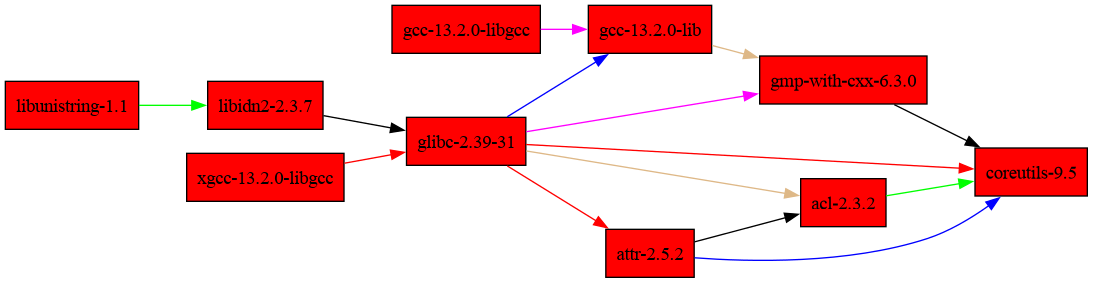
\includegraphics[width=0.4\textwidth]{figures/coreutils.png}
    \caption{The dependency graph of the coreutils package, generated by \texttt{nix-store --query --graph \$(nix build nixpkgs\#coreutils --print-out-paths) | dot -Tpng -ocoreutils.png}}
    \label{fig:nix-graph}
\end{figure}

Package derivations for the Nix package manager are written in a domain specific language which is also called Nix.
Derivations are the ``build plans'' on how Nix should build a specific software, which resulting build artifacts should be stored where, what the inputs are and so forth.
There are several different phases during a build, which contain shell code that is being run one phase after the other.
Those phases default to a given behavior, depending on the build system used.
All phases can be overridden freely to give users a maximum of flexibility when building and packaging software for Nix.
The most important phases users will override are the \texttt{patchPhase}, \texttt{buildPhase}, \texttt{installPhase} and \texttt{checkPhase}.
During the build, a special bash variable \texttt{\$out} is set that contains the path to the target directory inside the Nix store.

As the Nix language is purely functional, evaluating and building the derivation with the same inputs, yields the same outputs.
This is a critical factor where Nix's reproducibility comes from.
Also, Nix builds are sandboxed so they can reproducibly be run, meaning that there is no internet access possible during a build.

Another benefit of the reproducibility are remote builds, so a build cluster can build packages and serve its Nix store to other machines running Nix.
The upstream build cluster is called ``hydra'' and Nix defaults to using the upstream hydra as a substituter, i.e. fetching all packages from the hydras binary cache.
When evaluating a derivation, Nix checks if the hashed path is existent in the local Nix store.
If it's not, then it queries all known binary caches, which per default is only the upstream binary cache, and fetches the path and all its dependent paths until the full closure is copied into the local Nix store.

Software patches are quite easy to apply in Nix.
One can simply provide a list of \texttt{.patch} files inside the Nix file describing a derivation, Nix will then include the patch files in the calculation of the hash.
This new store path can probably not be found in the upstream binary cache, so Nix will fall back to building from source.
Nix also provides overriding all inputs freely, so every package can be flexibly adjusted to the users needs.


\subsection{preCICE}

preCICE (Precise Code Interaction Coupling Environment) is an open-source software library designed to facilitate the coupling of different computational simulation softwares.
It provides an interface that allows different simulation tools to exchange data and work together in a collaborative manner, enabling multi-physics as well as multi-scale simulations.

Many scientific simulations require complex combinations of multiple solvers, each specialized in a particular aspect of the problem.
For example, in fluid-structure interaction problems, where fluid flow interacts with deformable structures, separate solvers can be used to model the fluid dynamics and structural mechanics.
preCICE acts as a bridge between all solvers participating in the simulation, allowing them to exchange data and synchronize their computations.

preCICE offers a flexible and generic framework for coupling simulations.
It supports a wide range of solvers, including finite element, finite volume, and particle-based methods.
The library provides methods for interpolating data between meshes, managing communication between solvers, and handling time stepping and convergence.
It can handle different types of coupling scenarios, such as one-way or bidirectional couplings, loose or tight couplings, and static or dynamic meshes.
The core principle of preCICE's functionality is shown visually in Fig. \ref{fig:precice}.

\begin{figure}
    \centering
    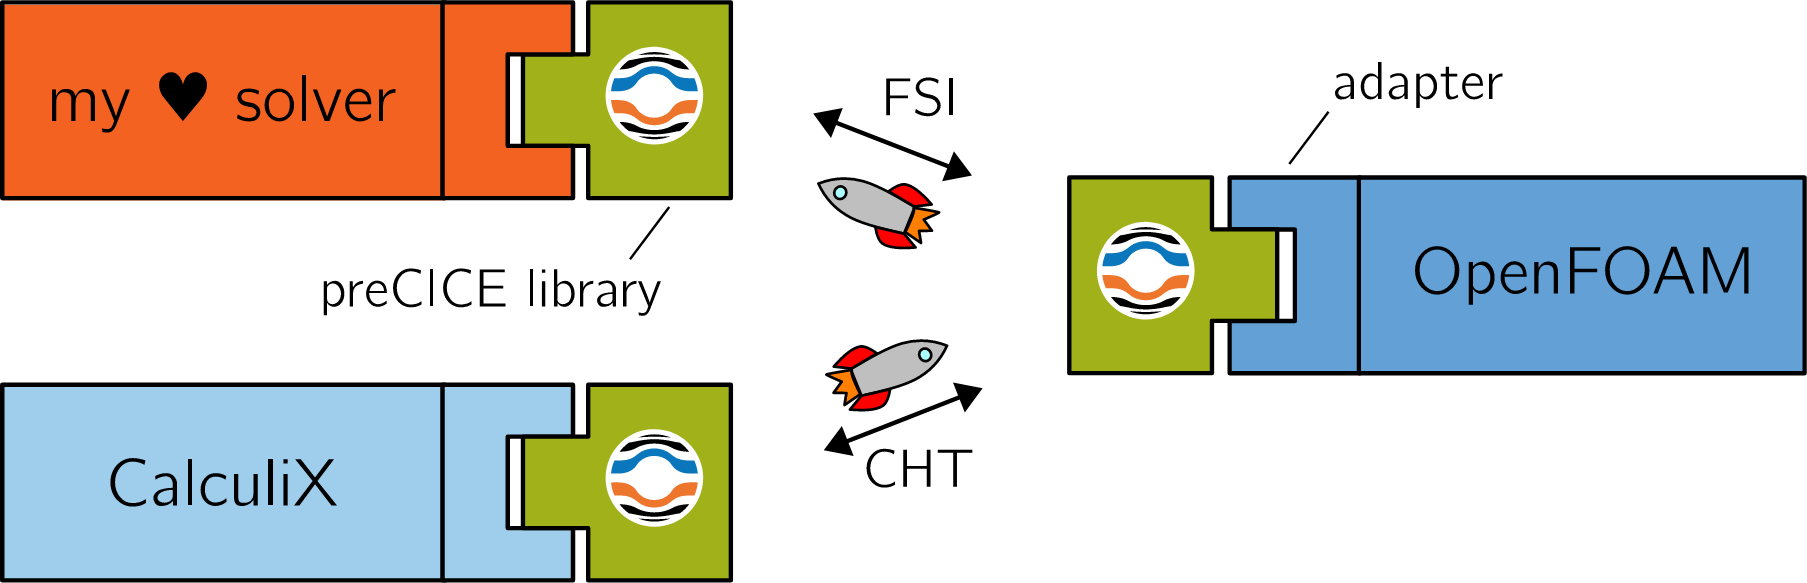
\includegraphics[width=0.5\textwidth]{figures/precice.png}
    \caption{A visual representation on how preCICE works in principle, see: \url{https://precice.org}}
    \label{fig:precice}
\end{figure}

One main idea behind preCICE is to enable the combination of existing simulation tools without requiring significant modifications to their original source code.
Instead, preCICE provides an abstraction layer that sits between the individual solvers, allowing them to communicate and exchange data efficiently.
This approach promotes code reusability and reduces the effort required for coupling simulations.

preCICE is an open-source project, which means its source code is freely available and can be modified and distributed by the community.
This fosters collaboration and encourages the development of new features and improvements by researchers and engineers worldwide.

Overall, preCICE simplifies the process of coupling different simulation programs, enabling the simulation of complex multi-physics problems.
It promotes interoperability, code reusability, and collaboration, making it a valuable tool in various engineering and scientific domains.

\section{Case study}

To see how well Nix can be used to build and package scientific software reliably and reproducibly, we conduct a case study in the context of the latest preCICE distribution~\cite{preciceDistribution}, which is currently preCICE \texttt{v2211.0}.
The preCICE distribution consists out of the preCICE core library, as well as some tools, bindings, adapters, tutorials, the website and documentation, and the preCICE VM\footnote{\url{https://precice.org/installation-distribution.html}}.
Table \ref{table:label-distribution} shows an overview over all packages provided by the preCICE distribution and their respected versions.

\begin{figure*}[!t]
  \normalsize
  \caption{Overview of preCICE distribution}
  \label{table:label-distribution}
  \centering
  \begin{tabular}{|c|c|c|c|}
    \hline
    \bfseries Package & \bfseries Type & \bfseries Build System & \bfseries Version \\
    \hline
    precice & library & cmake & 2.5.0 \\
    \hline
    fortran-module & bindings & make & 9e3f405 \\
    \hline
    julia & bindings & julia & v2.5.0 \\
    \hline
    matlab & bindings & matlab build script & v2.5.0.0 \\
    \hline
    pyprecice & bindings & setup.py & 2.5.0.1 \\
    \hline
    config-visualizer & tooling & setup.py & 60f2165 \\
    \hline
    precice-aste & adapter & cmake & 3.0.0 \\
    \hline
    dealii & solver & cmake & 9.4.1 \\
    \hline
    precice-dealii-adapter & adapter & cmake & dbb25bea \\
    \hline
    precice-calculix-adapter & adapter & makefile & 2.20 \\
    \hline
    fenics & solver & cmake + setup.py & 2019.1.0 \\
    \hline
    precice-fenics-adapter & adapter & setup.py & 1.4.0 \\
    \hline
    precice-dune & adapter & scripts + cmake & 2.8.0 \\
    \hline
    Dune-fem & library & setup.py & 2.8.0.0 \\
    \hline
    code-aster & solver & custom build system in python & 14.6.0 \\
    \hline
    openfoam & solver & wmake/Allwmake & 2206 \\
    \hline
    openfoam-adapter & adapter & wmake/Allwmake & 1.2.1 \\
    \hline
    Precice-su2 & solver + adapter & patch script + autoconf & 6.0.0 \\
    \hline
    Nutils & library & setup.py & 7.0.0 \\
    \hline
  \end{tabular}
\end{figure*}


We are mainly interested in the tools, adapters including their solvers and the preCICE VM.
For each of these entities, we present possible challenges, how to circumvent those and also comment on how software can be designed to make it as easy as possible for other users to build and package the software in question.

\subsection{preCICE}

The preCICE library itself is already available in the nixpkgs repository, so we don't have to package the software.
Looking at the package definition and the preCICE source code, the library is quite easy to build and package as it uses CMake as a build system.

\subsection{Tools}

The preCICE distribution comes with a few tools that ease working with preCICE.
They are mainly meant for debugging and visualizing several aspects of preCICE and preCICE configuration files.

\subsubsection{ASTE}

This package is a collection of tools which help in development of new adapters.
It stands for Artificial Solver Testing Environment, so it allows for debugging adapter mapping setups and other similar tasks.

ASTE\footnote{\url{https://github.com/precice/aste}} needs VTK9\footnote{\url{https://vtk.org/}}, a visualization toolkit, which is built without python support in the nixpkgs repository to reduce compilation time.
However, this feature is needed for ASTE.
As already mentioned, Nix allows easy overriding of inputs, so in this case, we can look at the package definition of VTK.
The parameter \texttt{enablePython} can simply be set to \texttt{true}, then we also need to supply the version of python we want to compile against, so in our case \texttt{python = python3;}.

After enabling python support in VTK, the package can be built without further modifications.

Only for testing, we additionally need to replace the absolute paths to \texttt{/bin/bash} and \texttt{/usr/bin/time}, then all tests succeed without any problems.

\subsubsection{config-visualizer}

The precice-config-visualizer\footnote{\url{https://github.com/precice/config-visualizer}} package can be used to generate images that represent a specified preCICE config file to check graphically what is configured in the file.

This tool is already packaged upstream, so we can just use it.
As it is a python package, it is quite easy to build with Nix, so the package definition is straight forward.

\subsection{Bindings}

Bindings are used to offer interfaces to other programming languages.

\subsubsection{python-bindings}

The \texttt{pyprecice} package is already available upstream, however it is broken and does not compile as it is not able to find the python module \texttt{pkgconfig}.
After adding this single dependency as an input to the package definition, the python package builds and can be used as expected.

\subsubsection{Julia-bindings}

Julia~\cite{bezanson2017julia} support in NixOS is currently still in its early stages and cannot be declaratively be defined by Nix\footnote{\url{https://github.com/NixOS/nixpkgs/issues/20649}}.

\subsection{Adapters}

A preCICE distribution comes bundled with several adapters, which are currently not in the upstream nixpkgs repository.
Many of the adapters use solvers that aren't packaged in the upstream repo as well, so in order to get the adapters to work, these also have to be packaged and sometimes patched.

\subsubsection{CalculiX}

The preCICE adapter for CSM code CalculiX~\cite{Uekermann2017_Adapters}, requires the original CalculiX source code and provides a new Makefile in the adapter repository.
By default, this Makefile expects the source code to reside in \texttt{\$HOME}, but it's possible to override this location with a make variable.
It then builds the original code and the adapter code together, which results in a combined binary.

The Makefile also has hard-coded dependency location for \texttt{SPOOLES}, \texttt{ARPACK} and \texttt{YAML} so these need to be replaced with the equivalent \texttt{pkg-config} calls, because Nix doesn't have these dependencies at the hard-coded locations, and generally only finds dependencies with \texttt{pkg-config}.
Additionally, there is no \texttt{install} target provided by the Makefile so the resulting binary needs to be installed manually by copying it to \texttt{\$out}.\\

\subsubsection{code\_aster}

The code\_aster preCICE adapter~\cite{Uekermann2017_Adapters} is a python file that needs to be placed in the code-aster lib directory.
For this, the code\_aster solver needs to be packaged at the latest stable version 14.6.
It uses a custom build system based on a \texttt{setup.py} file, that invokes build and install phases for dependencies and in the end for the solver itself.

The stable package also distributes the dependencies as pinned tarballs.
On Nix almost none of these dependencies, complete the build stage with the \texttt{setup.py}, so we need to pull them out, package them separately as Nix packages and configured the build system with a \texttt{setup.cfg}.
In this file, we are able to disable the installation of the pinned dependencies and provide paths to the dependencies instead.

With this approach, we disable HDF5, which is already packaged in the upstream nixpkgs repository, even at the required version 5.1.10.
HDF5 is packaged with multiple outputs.
One package, \texttt{out}, contains the libraries and binaries and another, \texttt{dev} contains the header files, this is, because most of the time, users installing HDF5 only need the libraries and binaries, and it helps to reduce installation size of this rather large package.
Additionally, code\_aster requires medfile and scotch, which are both available upstream and can be used as a dependency.

Another dependency, which is also provided by code\_aster is metis, which partially builds, so we do not replace this dependency, but we need to fix the second part of the build, which includes the metis programs like gpmetis, ndmetis, mpmetis and more.
The issue is that in the \texttt{CMakeLists.txt} for the metis programs \texttt{link\_directories} is hard-coded to \texttt{/home/karypis/local/lib}.
After removing this line, it also installs, so to resolve this issue in the buildPhase, we unpack the metis tarball, remove this line with \texttt{sed} and then repack the directory.

The last 2 dependencies, are not available and need to be packaged, this includes mumps and tfel, also known as mfront.

Mumps builds using a Makefile and can be configured using Makefile.inc, by default it provides a couple of these configurations for systems like Ubuntu, so we use one of these provided configuration files to write our own custom config file.
It defines the location for dependencies like scotch, metis, parmetis, liblapack, blas, scalapack and blacs.
Almost all the dependencies, are available upstream, but we need to recompile scotch with additional build flags, \texttt{scotch ptscotch esmumps ptesmumps} using Nix overrideAttrs feature.
For packaging blacs, which also uses a Makefile, we configure the build using a custom \texttt{Bmake.inc} file, which is used to set compiler flags, the path to the mpi and bash installation.

The last missing dependency for code\_aster, tfel, uses CMake as a build system which makes packaging it trivial with Nix and we only have to set a couple of CMake flags.

After successfully packaging all dependencies, the build phase of code\_aster completes, but the installation part has another issue, that also affects new versions of Ubuntu and other distributions which use a python version greater than 3.9.
There is a forum post without any resolution from the developers or the community, so we need to manually patch the bug.

The issue is that the custom build system does not correctly calculate the python site-packages directory because it unconditionally slices the first 3 chars from \texttt{sys.version}, which works if your version is 3.9.x but not with 3.10.x because then the code calculates \texttt{lib64/python3.1/site-packages} rather than the expected \texttt{lib64/python3.10/site-packages}.

After patching this bug code\_aster successfully installed into \texttt{\$out/14.6/}, so we move around some files until we have a valid directory structure with \texttt{\$out/bin}, \texttt{\$out/lib} and we provide symlinks for \texttt{\$out/14.6/} and \texttt{\$out/stable/} as code\_aster expects configuration files in these directories.

Last but not least, we can copy the code\_aster adapter at the required location which concludes this adapter installation.\\

\subsubsection{deal.II}

In order to package this adapter, we first need to package deal.II~\cite{dealII95}, which uses CMake as build system and works without any adjustments.
The same applies for the adapter, which also uses CMake and needs preCICE as a dependency.
When supplied with the inputs, the adapter builds without any problems.
As an example for the Nix language, you can see the abbreviated Nix code for the dealii.II adapter in Fig. \ref{lst:dealii-adapter-nix}.\\

\begin{figure*}
    \normalsize
    \begin{minted}{nix}
{ lib, stdenv, fetchFromGitHub, cmake,
  precice, dealii, enable3d ? false }:

stdenv.mkDerivation rec {
  pname = "precice-dealii-adapter";
  version = "unstable-2022-09-23";

  src = fetchFromGitHub {
    owner = "precice";
    repo = "dealii-adapter";
    rev = "dbb25...8367c";
    sha256 = "sha256-pPQ2...2jlflgUE=";
  };

  nativeBuildInputs = [ cmake ];
  buildInputs = [ precice dealii ];

  cmakeFlags = lib.optionals enable3d [
    "-DDIM=3"
  ];

  installPhase = ''
    mkdir -p $out/bin
    cp elasticity $out/bin/elasticity
  '';
}
    \end{minted}
    \caption{A sample of Nix code used to package the dealii-adapter, see: \url{https://github.com/precice/dealii-adapter/}}
    \label{lst:dealii-adapter-nix}
    \hrulefill
    \vspace*{4pt}
\end{figure*}

\subsubsection{DUNE}

The DUNE~\cite{bastian2020dune} package uses a combination of CMake files and custom build scripts which makes the build process quite tedious.
This might be an issue because of the ongoing migration to CMake from autotools and might be resolved in the future.

It's also a minor issue that the dune-project is a collection of repositories rather than a monorepository, because users have to correctly clone all repositories so the build system finds all relevant information.
We clone all of the required dune repos into a directory and additionally clone the adapter into the same directory.

For the build and install, process we need to manually set \texttt{\$DUNE\_CONTROL\_PATH} and \texttt{\$DUNE\_PY\_DIR} environment variables, both variables also need to be set at runtime.
Additionally, we need to patch the python install process because the current CMake file that handles this install tries to access the internet with \texttt{pip install} which isn't allowed in Nix' sandboxed builds.
Therefore, we need to patch this \texttt{pip} command with the options \texttt{--no-build-isolation --no-cache-dir --no-index --no-deps} and we need to remove the \texttt{--upgrade} option.\\

\subsubsection{FEniCS}

We are explicitly referring to the legacy version of FEniCS~\cite{fenics} here, not the newer and still experimental FEniCSx.
This adapter~\cite{Rodenberg2021} uses the open source computing platform FEniCS, which is already packaged within nixpkgs, to provide preCICE support.

Although it is available, not all features the adapter needs are enabled, including PETSc support.
To fix this, we need to package PETSc4py, which provides python bindings for PETSc and is not present in the upstream nixpkgs repository.
The build process is possible without any issues, because it uses the internal \texttt{buildPythonApplication} build tool, but we need to add the additional build optional \texttt{build\_src --force} because the cython code needs to be rebuilt.
We also aren't able to enable tests for this package because tests depend on OpenMPI and the network, which isn't available within the Nix build sandbox.

After this, we can specify PETSc4py as dependency for FEniCS and can enable support for this feature.

Building the adapter with Nix is now possible with \texttt{buildPythonPackage} and doesn't require any special workarounds.
A majority of the \texttt{pytest} ran successfully, but two tests failed inside the Nix sandbox, which means all tests needed to be disabled.\\

\subsubsection{OpenFOAM}

There are two flavors of OpenFOAM, we are referring to the OpenFOAM fork of OpenCFD Ltd\footnote{\url{https://www.openfoam.com/}}.

OpenFOAM uses its own custom build system called \texttt{wmake} which is sometimes called with a wrapper script called \texttt{Allwmake}.
The build system sets 36 environment variables that are set by wmake, one step at a time by checking several parameters, e.g. the cpu architecture or the location of the source code, and concatenating some other environment variables together.

Allwmake and wmake rely on these environment variables to be set, as otherwise the tools will exit with a warning.
During runtime, before running any OpenFOAM commands, a small wrapper script has to be started that sets all relevant environment variables, or a user has to manually source a file inside the installation directory of OpenFOAM.
OpenFOAM uses modules for extensibility and flexibility which need the source code of OpenFOAM and also require wmake as a build tool.

For Nix, these properties are rather unfortunate.
To compile OpenFOAM with Nix, we first need to patch the shebangs\footnote{\url{https://foldoc.org/shebang}} of wmake to make it run during the build.
Secondly, we render a shell script we call \texttt{set-openfoam-vars} that exports all necessary environment variables to the current shell session.
At the time of writing, all parameters such as the processor architecture are hard-coded for simplicity reasons but could be parametrized based on the Nix inputs to allow for optimized builds.
During the buildPhase, the rendered script will be sourced to set all variables, e.g. so the \texttt{OPENFOAM\_SRC\_PATH} points to \texttt{/build/openfoam} which is the default location for Nix builds inside the sandbox.
After sourcing the script, the single command \texttt{./Allwmake -j -q} is sufficient to start the build.

The installPhase then simply copies the necessary files and directories to \texttt{\$out}, replaces the mock \texttt{OPENFOAM\_SRC\_PATH} by the value of \texttt{\$out} and creates a wrapper for the \texttt{openfoam} shell script.

As the preCICE OpenFOAM-adapter~\cite{OpenFOAMpreCICE} is an OpenFOAM module, the derivation of the adapter needs OpenFOAM and wmake as build inputs.
The correct environment variables have to be set again, but this is rather easy now, as we have the \texttt{set-openfoam-vars} script that we can simply source during the buildPhase.
The last thing we need to change before launching the build with Allwmake is to set the target directory for the adapter.
A single shared library that can be copied to \texttt{\$out/lib/} is the only output for this build.

Debug and timing modes for the adapter can simply be enabled by setting the \texttt{debugMode} and \texttt{enableTimings} inputs to the derivation to true.

OpenFOAM is available on Spack and EasyBuild which both patch the OpenFOAM source files as those tools also have to set environment variables to make a build compatible with wmake.\\

\subsubsection{su2-adapter}

This package is a preCICE adapter~\cite{Uekermann2017_Adapters} for the CFD code SU2 and extends the original SU2 source code by patching the files.
For this, the adapter provides a custom script that needs to be executed before the build phase.
Nix offers the patchPhase which allows us to run the script in this phase and patch the original source, after that the \texttt{stdenv} automatically recognizes that the repository uses autotools for building the software and runs the configurePhase.

We additionally needed to add the two configureFlags \texttt{--with-include} and \texttt{--with-lib} to the preCICE install directory because otherwise autoconf does not find the preCICE installation directory.

\subsection{preCICE VM}

The current preCICE VM is built on top of Vagrant\footnote{\url{https://www.vagrantup.com/}} using Ubuntu as a base image.
When it is run for the first time, it further installs software, compiles programs and the preCICE tutorials\footnote{\url{https://github.com/precice/tutorials/}}.
This inherently breaks reproducibility as the VM fetches files from the internet that are at this very point in time the ``latest'' version, e.g. the \texttt{main} branch of the preCICE repository.

Nix comes with the built-in functionality of producing qemu\footnote{\url{https://www.qemu.org/}} VM images.
We used Nix to define a VM image with NixOS as a base, that can be built reproducibly.
The image contains all the adapters and solvers from the case study and some additional custom tools that can only be seen in the official, like the \texttt{preciceToPNG} command.
Also, we generate an iso and a Vagrant VirtualBox file of the VM as additional outputs.

Most of the functionality that can be found in the official VM is also available in our NixOS VM and preCICE tutorials, like the \textit{perpendicular-flap} can be run successfully.

\subsection{Discussion}

After detailing the challenges of building and packaging each solver and their respective adapter, we want to discuss some common points between these scientific software packages.
preCICE, as a multi-component research software, covers many different simulation codes and therefore provides a good overview over different kinds of packages, making this case study representative for multi-component research software.\\

Generally speaking, there are major gaps regarding the ability to successfully package the software between each different software solution that can be traced back to the build system.
Custom build systems require an disproportional amount of additional work to make them runnable on any system.
OpenFOAM and Allwmake are prime examples of these issues because now package managers have to understand a whole new build system for exactly one package in order to successfully package it and make it easily available to users.
It is also worth mentioning that writing your own custom build system, requires additional time to maintain this build system, which could have been spent working on the software itself.
Packages that use common, industry proven package managers, like CMake and autotools make it easier for developers of the software to build their software as well as package managers to package it.
These build tools, generally also provide interfaces for dependency management which can be used to tell users and package maintainers which dependencies are needed, and it is usually better than only documenting required dependencies, because documentation needs to be kept in sync with the underlying code.
They also generally already provide proven interfaces for configuring packages with additional features, and these also might be self documenting.

The authors of the xSDK\footnote{\url{https://xsdk.info/}} came to a very similar conclusion.
Their goal is to ``identify, adapt, and adopt best practices in software engineering''~\cite{xsdk-website} and ``to provide the foundation of this extensible scientific software ecosystem''~\cite{xsdk-website}.
To achieve this they provide a list of package policies~\cite{xSDK2023}, which for example specifies as mandatory policy that packages ``must support portable installation through Spack''~\cite{xSDK2023} and that all packages ``should have a build system that is appropriate for the language''~\cite{xSDK2023}, which includes CMake and autoconf as examples.
If a package supports all these policies, they can be added to the growing list of packages in the xSDK, which currently among other things include PETSc, deal.ii and preCICE.
These packages are already part of nixpkgs, or it is easy to provide a package for them because they support portable installation, meaning installation into custom prefixes like nix store paths, and common build systems like CMake and autoconf.

Another finding is, that is also addressed in xSDK through portable installations, is the requirement to install software to be installed into \texttt{\$HOME} or requires files to be located at a specific location on your file system.
Most of the time, it is possible to work around this, but there are already available solutions for dependency management.
Both, the CalculiX-adapter and SU2-adapter do require the original source code to be present as they add new features on top or patch the source code.
The current solution of the user cloning the code at the specific location works, but it might be better to look into submodules because that also allows the developers to pin the version more easily rather than documenting it, as that could more easily lead to user error, when they try to package and install the adapters.

Additionally, hard-coding libraries to \texttt{/usr/lib} and \texttt{/usr/include} might work on one distribution, but might make it hard or even impossible to install a package on a different distribution or even a later version of the same distribution.
Solutions like \texttt{pkg-config} that can be configured, so it finds libraries outside the common paths, should always be preferred and work out of the box with the common paths like \texttt{/usr/lib}.

With Nix' dependency management, we can easily copy the package definitions we just wrote onto different systems, e.g., entirely different Linux distributions, and execute the build of the closures there.
Building the same closures yields the same outputs, this will also be described in section \ref{sec:nix-on-hpc}.

\section{Comparision}

This chapter defines metrics and uses these metrics to compare the Nix package manager~\cite{Dolstra_2004} with widely used HPC package managers Spack~\cite{Gamblin_2015} and EasyBuild~\cite{Geimer_2014}.

\subsection{Metrics definition}

In this section, we define all metrics used in the comparison of the selected package managers.
The metrics are grouped with related metrics.\\

\subsubsection{Overview}
The first few metrics are grouped as Overview, where we present some basic stats about each package manager.
First, we look at the number of available packages, then at the number of unique packages, meaning all packages minus packages that are available at different versions and last we compare how packages can be implemented.\\

\subsubsection{Installation}
In this section, we look at the installation of all 3 package managers, how they can be updated and if root permissions are needed to either install it or later install packages.\\

\subsubsection{Usage}
In Usage, we present basic usages of the package managers.
We show how you can search for packages, install software, install software with a specific version, install software at a specific point in time, specify the compiler that is used to install a piece of software and last we show how to build optimized software for your architecture.\\

\subsubsection{Reproducibility}
Here we look into reproducibility of build software.
We first look into how the reproducibility is achieved, then if the architecture and cpu features are considered and latestly we look at the dependencies can affect reproducibility.\\

\subsubsection{Performance}
We will take a short look at the performance of the package manager and the resulting packages\\

\subsubsection{Testing}
Finally, we look into tests and see what features the package managers provide for validating that a package works as expected.

\subsection{Results}

This section presents the results we collected.
First we will provide a description and afterwards we will discuss the gathered results.\\

\subsubsection{Overview}

For the first set of metrics, we observed that in our comparison Nix provides the most packages with 83000 packages, 67000 of them unique, followed by Spack with around 7000 packages, 6000 of them unique.\footnote{\url{https://repology.org/repositories/statistics/total}}
Regarding EasyBuild, there are around 17000 and 3000 unique packages.\footnote{\url{https://docs.easybuild.io/release-notes/}}

While Nix has the most amount of packages, it is a general purpose package manager not specifically made for scientific software.
This means, that most of the packages are not focused on scientific software, but it still comes with important packages like HDF5 and mostly offers mpi support for those packages.

Spack and EasyBuild lay their focus more on the HPC/Simulation environment, so the main purpose of these package managers is to provide scientific software, but that also means that sometimes common packages, like openssl3.0 simply aren't available.

Both, Spack and EasyBuild, use python scripts to implement their packages, Nix on the other hand, uses with its own DSL.
Using a common language to define packages makes it easier for new people to get started packaging their own software because they might already be familiar with the language and generally, there is more documentation available for general purpose language, especially python.
The Nix DSL is only useful inside Nix and people looking to package their software for Nix, need to learn a new language that is only applicable within Nix.\\

\subsubsection{Installation}

Nix, the package manager, can be installed with a custom installation script.\footnote{\url{https://nixos.org/download.html\#download-nix}}
There are multiple ways to install it, with the Nix daemon, making it a multi-user installation, this installation requires root privileges for installation and installs it in \texttt{/nix}, after that normal users can use the Nix binary to communicate with a running daemon to download and install packages, this does not require root permissions.
The single user installation allows to setup the Nix package manager inside your home directory, this method does not require root for installation and usage.
The third way is to install Nix as part of NixOS and requires a new installation of the operating system, requires root for installation but not for usage.

Spack is being installed with git and can be cloned into any directory, which means it does not require root for installation and usage.\footnote{\url{https://spack.readthedocs.io/en/latest/getting_started.html\#installation}}

EasyBuild also has multiple ways to install it.\footnote{\url{https://docs.easybuild.io/installation/}}
It can be installed with \texttt{pip install} (or virtualenv/pipenv) and after that can be loaded with \texttt{module load EasyBuild}.
It can also be installed into a temporary directory using \texttt{pip} and afterwards properly installed with using the temporary installation to bootstrap an install into the latest release.
EasyBuild installation requires modifying \texttt{PATH}, \texttt{PYTHONPATH} and potentially \texttt{MODULEPATH} depending on the location, it is being installed in.
It also requires Tcl/C environment-modules or Tcl-only variant of environment modules or Lmod being installed and configured.
None the less EasyBuild can be installed without root privileges and generally can also be used without root, but EasyBuild has a package option called \texttt{osdependencies} with requires dependencies being installed on the operating system.
For example CMake (till 3.18) requires \texttt{openssl-devel}, \texttt{libssl-dev} and \texttt{libopenssl-devel} making it impossible to install for a normal user, if one of the above packages is not installed.
This also means that users can't install any package that requires the CMake build system without updating the package definitions.

Last but not least, updating the tools and their packages, is also widely different.
Nix has something that is called channels that need to be advanced upstream and after that users can update their local channels with \texttt{nix-channel --update}, or use the newer Nix flake technology which pins the inputs so users can choose freely when to update to which commit of the upstream nixpkgs repository.

Spack is being updated by fetching a new version of the local repository, which then can lead to merge conflicts if users change the provided package definitions.

EasyBuild can be updated using the \texttt{--install-latest-eb-release} the tool provides.\\

\subsubsection{Usage}

The basic usage of each tool is pretty similar.
All 3 package managers allow a user to query for a package than then can be installed.

Nix allows for downloading and installing software within the current shell session\footnote{\url{https://nix.dev/tutorials/first-steps/}}, that means that an only accessible within the shell and not actually installed on the system in the classical sense of making it available to multiple users of the system.
A user or an administrator can at any point \texttt{collect-garbage} and all packages not specified as installed system packages are being removed that includes packages installed in the current shell, as long as the shell session isn't still open.
If a user wants to install a specific software at a given version there are two main options made available by Nix.
Either there is an old package version definition provided by the packages, like \texttt{boost159} or a user can opt into overriding the package by overriding the \texttt{version} and the \texttt{src} \texttt{nix-shell -p 'precice.overrideAttrs(\_: \{ version = "2.4.0"; src = \ldots \} )'}, that will build the package given the specific source, which can be a remote tarball, revision in a repository or even a local directory.
With these options, users can override any aspect of the package definition, including the dependencies and even providing custom patches.
Each change to the package will trigger a new build because the input for the build was changed.

Spack and EasyBuild on the other hand, keep the old software versions in the specifications or keep the whole specification, so you can reinstall an old version by specifying the available version, for example, \texttt{spack install gcc@6.4.0}.\footnote{\url{https://spack.readthedocs.io/en/latest/basic_usage.html}}
If the required version is not available, you have to edit the current package definition and add the required version.
There is no elegant way of overriding the package in a command call and Spack even provides a command \texttt{spack edit} which does it in tree.
This can be an issue if you later want to update the git revision, as this might lead to merge conflicts as soon as you checkout a new revision, as described earlier.

To achieve reproducibility, it is necessary that we can install software from a previous revision of the packages.
Nix allows us to simply specify the channel revision we want to use to build our software, it then evaluates the requested packages and builds it.
This can easily be done without affecting the current system by specifying it in the shell command \texttt{nix-shell -p pan -I nixpkgs=pathToRevision/urlToTarball}, it now only uses this channel for building the requested package.
Spack, can achieve something similar by checking out your Spack version at a previous revision and then installing the package requested package, but this approach has a downside that it affects the whole Spack installation, and now also work with an older Spack tool.
On the other hand, EasyBuild, could be installed using pip at an earlier version, but it also offers something different called toolchains, which we will look at shortly.

Next, we look at how you can build a package with a specific compiler version.
The flexibility of Nix overrides allows different levels of rebuilds of packages with a specific compiler, you can either just rebuild the requested package with specific compiler, this for example rebuilds curl with clang8 \texttt{nix-shell -p '(curl.override \{ stdenv = clang8Stdenv;\})'} or you can rebuild the package and all required dependencies with a specific compiler by overriding the \texttt{stdenv} on nixpkgs level, \texttt{nix-build -E 'with (import <nixpkgs> \{ config.replaceStdenv = \{ pkgs \}: pkgs.clang8Stdenv; \}); curl'}.
This is possible because every c/c++/\ldots package, is build using the \texttt{stdenv} which defines the compiler and default compile flags.
While Nix provides a default stdenv, which is used to compile all packages, it is possible to override and replace the package with your another stdenv provided by nixpkgs, like the clang8Stdenv, you can write your own stdenv, or you can extend the current stdenv with flags.
By default, there are some useful helpers provided, like \texttt{makeStaticLibraries} which allows compiling any library as a static library, or \texttt{enableDebugging} which sets the compiler flags \texttt{-ggdb -Og} and can then be enabled on the package plus all dependencies.

Spack provides an easy way to specify the compiler using \texttt{spack install precice \%clang} and only requires a registered compiler, it can be a system compiler, or the compiler can be installed using Spack.\footnote{\url{https://spack.readthedocs.io/en/latest/basic_usage.html}}
On this note, Spack tooling and interface to override compilers, flags and more is way more user friendly and readable than using and invoking the Nix DSL within a one line command call.

EasyBuild has a whole different system, where packages have defined toolchains.\footnote{\url{https://docs.easybuild.io/common-toolchains/}}
A toolchain is a set of packages defined at a specific version and users can create their own toolchains.
For example, EasyBuild provides a foss toolchain which contains packages like, binutils, gcc, OpenMPI, openblas and more and packages are provided against a specific toolchain version like foss-2022b.
Packages are then provided with toolchains in mind and are never deleted, so installing a package with a different compiler can be achieved by selecting a different eb script with a different toolchain version.
On the other hand this results in a less elegant user flow, because if a user wants to install a package with a toolchain that isn't provided they have to fork a package definition and update the toolchain.\\

\subsubsection{Reproducibility}

\begin{figure}
    \centering
    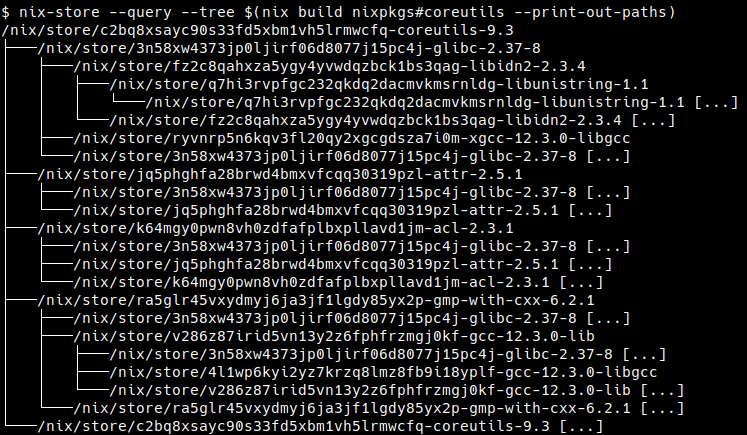
\includegraphics[width=0.4\textwidth]{figures/nix-tree.png}
    \caption{The dependency graph of the coreutils package, generated by \texttt{nix-store --query --tree \$(nix build nixpkgs\#coreutils --print-out-paths)}}
    \label{fig:nix-tree}
\end{figure}

As previously mentioned, Nix computes an output hash over all its inputs that is unique for this input, so if anything in the inputs changes, like the version of a dependency, the output hash changes resulting in a different software build.
This guarantees that given the same set of inputs, we are able to compile the same software, including it's dependency tree as you can see in Fig. \ref{fig:nix-tree}.
One thing to mention is, that Nix currently only builds generic architecture build, so the inputs of a derivation don't include any information about the architecture and/or compiler features.
Another thing to mention is, that all software in the \texttt{/nix/store} can only link back to the \texttt{/nix/store} itself.
Nix validates this for every package and breaks links than allowing links back to a file in the home directory or the directory that was used for building the software.
This is required, to guarantee the best possible reproducibly.

Spack does something similar to Nix where it adds hashes to each installation path, but also stores additional files inside the package installation which include the complete spec of the package than can later be used to reproducibly build the same package.~\cite{Gamblin_2015}.
It also does something that Nix, currently doesn't support, which is it storing the architecture and cpu features that are used in this build, that way it can provide binary packages that are optimized for specific CPUs.
None the less it has one problem that Nix doesn't have: it allows packages to link back into system dependencies, for example, while building hpl-2.3 using a gcc 12.2.0 compiled with Spack we see the usage of the following system dependencies.
\begin{itemize}
  \item libm.so
  \item libc.so
  \item libdl.so
  \item libnl-3.so
  \item libnl-route-3.so
  \item librt.so
  \item libutil.so
  \item libpthread.so
\end{itemize}
Most of these dependencies are stable, and usually don't change on a system update, but it also means that it simply can't guarantee the best possible reproducibility and it gets worse if the system compiler was used rather than a compiler build from scratch using Spack.

EasyBuild does achieve reproducibility with its toolchains and the approach to keep old package definitions, meaning that they also keep old dependency definitions and each dependency is pinned at a specific version~\cite{Geimer_2014}.
Regarding, CPU architecture and features, EasyBuild does not do generic builds by default but rather prioritizes the idea of optimizing for a specific system, meaning defaulting to \texttt{-march=native} for all packages and it has to manually be disabled~\footnote{\url{https://docs.easybuild.io/controlling-compiler-optimization-flags/\#controlling\_compiler\_optimization\_flags\_optarch\_default}}.
This leads to inherently impure and irreproducible builds as building the same easyconfig on two different host/architectures results in different binaries.
On the other hand, the already mentioned option for \texttt{osdependencies} goes against the reproducibility idea, because any os dependency is not managed by the package manager and might change at any point.
This leads to the problem of binaries linking back to the operating system \texttt{/usr/lib}, that Spack also has.
For example a build of curl, uses libssl, libcrypto, libz, libm and libc, all of which are provided by the operating system, and for EasyBuild it includes libraries that change more frequently like libssl, libcrypto and libz.\\

\subsubsection{Performance}

With Nix' possibility to override stdenv it is also possible to set custom compiler flags and Nix provides an option \texttt{impureUseNativeOptimizations} to build packages optimized for your hardware, using the \texttt{-march=native} compiler flag, it can then be applied to the package, that is being installed, or every dependency in the dependency graph.~\footnote{\url{https://nixos.wiki/wiki/Build_flags}}
Nix can guarantee these compiler flags for every dependency because Nix wraps its compiler binaries in scripts, which then means it has more control over them and packages can not remove any flags by clearing environment variables.
The advantage of overriding the stdenv is that every package in a dependency tree can be optimized which might lead to better overall performance of packages, but it also has the downside that every package needs to be rebuild which might take several days, for example preCICE required a rebuild of 1500 packages, which took 2 days on an high-performance computing (HPC) cluster (2x AMD EPYC 7702).
So it might be sufficient to optimize only the package, which is easily possible with \texttt{(package.override)} like shown before or additionally optimize its direct dependencies, which is possible but more time-consuming to do, because one has to manually override each dependency.

Spack also allows to override cflags, using \texttt{spack install \ldots cflags='-march=native'}, so the package is then being optimized.
By setting cflags with \texttt{==}, the cflags are also applied to the dependencies, causing them to be rebuilt.\footnote{\url{https://spack.readthedocs.io/en/latest/basic_usage.html\#compiler-flags}}
Additionally, there is a way to define flags for a specific registered compiler, but these are only respected by CMake and autotools packages.
Also, a package might also have unavoidable system dependencies and are not optimized, which might impact performance negatively.

Like previously mentioned, EasyBuild applies \texttt{-march=native} by default, but you can further customize your compiler flags using \texttt{\$CFLAGS}, \texttt{\$CXXFLAGS}, \texttt{\$FFLAGS}, \texttt{\$F90FLAGS}.
It also has the same problem as Spack that it might have unavoidable unoptimized system package which might impact performance negatively.\\

\subsubsection{Testing}

We also shortly look at the capabilities of the package managers to run test and evaluate the built packages.
Nix has something that is called a checkPhase which can be run for each package after being built.
There are sane defaults for all available build systems, like \texttt{make test} or \texttt{ctest} for makefiles and CMake, \texttt{cargo check} and \texttt{cargo test} for rust packages, \texttt{go test} for go packages and \texttt{pytest} for python packages and more.
By default, this checkPhase is not enabled for every build system, like the \texttt{stdenv} build system, which is responsible for make, CMake and similar, does not enable it but the \texttt{go}, \texttt{rust} and \texttt{python} build system does.
For these build systems, package maintainers have to manually disable the check phase or they can override the check phase if the tests aren't working out of the box and make the needed adjustments to resolve the issues.

Spack has something similar, but its not enabled by default, and users, not package maintainers, has to manually specify that they want to run test on installing the package with \texttt{--test=root}.

EasyBuild on the other hand does not offer this feature but has another feature called sanity checks, where EasyBuild ensures that paths and or binaries, specified by a package maintainer inside the package definition, are successfully installed.

Additionally, Nix offers a way for testing multiple packages in combination and or with a specific network setup by providing a way to write your own tests.
These tests are then running inside isolated qemu virtual machines and users are able to start as many VMs as they need and define the set of commands that need to run on each of the so-called nodes.
The tests are pythons scripts, and it is possible to wait until systemd targets are running, until ports are available or wait until commands are completed and compare the output and status codes.

\section{Nix on HPC}\label{sec:nix-on-hpc}

High-performance computing refers to the utilization of powerful computational resources to tackle computationally intensive scientific problems.
It involves the parallel execution of tasks across multiple computing units, also called nodes in this context, enabling researchers to perform complex simulations, data analysis, and modeling at large scales.
HPC systems, such as clusters, supercomputers, and cloud-based infrastructures, usually offer immense processing power, storage capacity, and specialized hardware, supporting scientific research across various domains\footnote{\url{https://www.ibm.com/topics/hpc}}.

In many HPC environments, the \texttt{module} system is being used to load different pieces of software from a local repository of available softwares, such as compilers and different message passing interfaces (MPI).
With the module command, different users can use different software or different versions of the same software at the same time without interfering with each other.
One major drawback here is, that without further configuration, users can only load software modules that were previously installed into the cluster by the clusters administrators, so any other software that is needed for a simulation, including its dependencies, have to be compiled by the users that want to conduct an experiment.
Sometimes, this can be quite hard, as some software expects libraries or other software artifacts at some hard-coded location as \texttt{/usr/lib/\ldots}\footnote{\url{https://hpc-wiki.info/hpc/Modules}}.

As mentioned, Nix uses the Nix store, which lies in \texttt{/nix/store} by default and all software artifacts are linked against libraries inside the Nix store.
So if there is no such path as \texttt{/nix/store} on the HPC clusters filesystem, all software would need to be recompiled as all links and paths inside the binaries would point to a non existent location.
We'd need administrator rights to be allowed to setup the Nix store globally on the cluster and to install Nix globally for all users.
However, Nix supports a Linux kernel feature called user namespaces, which is a form of kernel based isolation of resources and other attributes like user ids\footnote{\url{https://www.man7.org/linux/man-pages/man7/user_namespaces.7.html}}.

Using namespaces, it is possible for the Nix package manager to mount an arbitrary user-writable location to \texttt{/nix/store} inside a user namespace, so all programs running in that namespace can access the Nix store as if it would actually be installed under the default store path.
Another challenge is to get Nix to work without the needed libraries that can usually be found inside the Nix store, leading to a bootstrapping problem.
We can simply use a statically compiled version the Nix package manager, however, to circumvent this problem.
In our repository, we provide a setup bash script that simplifies download, configuration and installation of the static Nix binary which can then be used to easily build and access the solvers adapters and the preCICE VM.

After installing Nix on HPC, we were able to produce the same binary output for the adapters and solvers as we built on our local machines as well as within the preCICE VM\footnote{The sha256 hashes of the resulting outputs were compared and matched.}

\section{Conclusion and Outlook}

In conclusion, the case study was a success, as it has shown that packaging of scientific software with Nix is possible, but it isn't as trivial as expected.
Once the software is packaged, it is quite easy to be used and combined in environments with other packaged softwares without conflicts.
The packaged adapters and solvers work well together with the preCICE library and simulations can be run successfully, so this specific case study has shown the potential of Nix in the domain of scientific software.
More research has to be done on the topic, yet we are positive about possible future results in Nix abilities and its flexibility in similar domains.

The majority of the packages required some solution for a fundamental issue within the scientific software or its build system that isn't solvable for none experienced Nix users, which makes it hard for people to use it even for their own software.
Nix itself also is partly at fault, because of its unique nature, that every piece of software lies within \texttt{/nix/store} and that each store path is its own-isolated tree based on the Filesystem Hierarchy Standard (FHS).
But it is worth mentioning that not only Nix would benefit from more streamlined build systems and packaging, because both Spack and EasyBuild do something similar for their packages, where each package also lies in its own FHS.
The work of the xSDK people and their policy might be a step in the right direction but looking at the current list of software that is available within the latest xSDK release, 26 libraries, indicates that it is an uphill battle that might take several more years, especially if we consider that the first release happened in 2016.
We have also seen, that the current HPC solutions, Spack and EasyBuild make it somewhat possible to reproducibly build software but not to the degree in which Nix allows it.
That is because they focus on flexibility of installing packages.
Spacks way of allowing users to change the compiler of a package, easily enable additional features on installation, override cflags and more advanced features, for example regarding mpi, shows that the Nix tooling needs more work or a layer on top that strips away the uniqueness of the DSL for something more user- and beginner-friendly.

Lastly we looked at Nix on HPC and have seen that it's possible to get it running, and we are able to run simulations on one node, so we currently assume that with the correct networking setup it should be possible to run a simulation across multiple nodes.
It is currently not ideally solved on getting Nix running on HPC as a single user installation, so this can be improved in the future.

The Nix code for the packages for the case study on the preCICE adapters, solvers and the preCICE VM is available online in a git repository at \url{https://github.com/precice/nix-packages/}.
Also the \texttt{setup.sh} and \texttt{clean.sh} scripts used to install Nix on HPC can be found there.\\


While this case study and this comparison has provided valuable insights into the topic of reproducible software, there are still numerous unanswered questions that merit further investigation.
This includes a full evaluation if there are performance improvements using a full impure system rebuild, with \texttt{-march=native} compared to only rebuilding the package at hand like we suspect.
It would also be interesting to look at trying to reproduce a nixpkgs commit from 10 years ago, and if there might be issues and incompatibilities with newer Nix versions, which currently get released in a 6 weeks time windows.

Last but not least, it would be interesting to investigate Nix and NixOS on HPC even more.
It would be interesting to see how an HPC cluster completely build on NixOS could improve maintaining the HPC cluster, with slurm already being available as a nixpkgs package and module providing a systemd service.

Finally, it would be interesting to investigate a nix store that is shared between users and how it might optimize the amount of storage needed for a cluster as each user is not required to rebuild the same package in their respective home directories.

This summary shows, how diverse and complex Nix is, and how much more opportunities there are to be researched in the future.

\nocite{*}
\bibliographystyle{eceasst}
\bibliography{paper}

\end{document}
